% Abstract set-membership schematic; boxes carry no metric/geometric meaning.
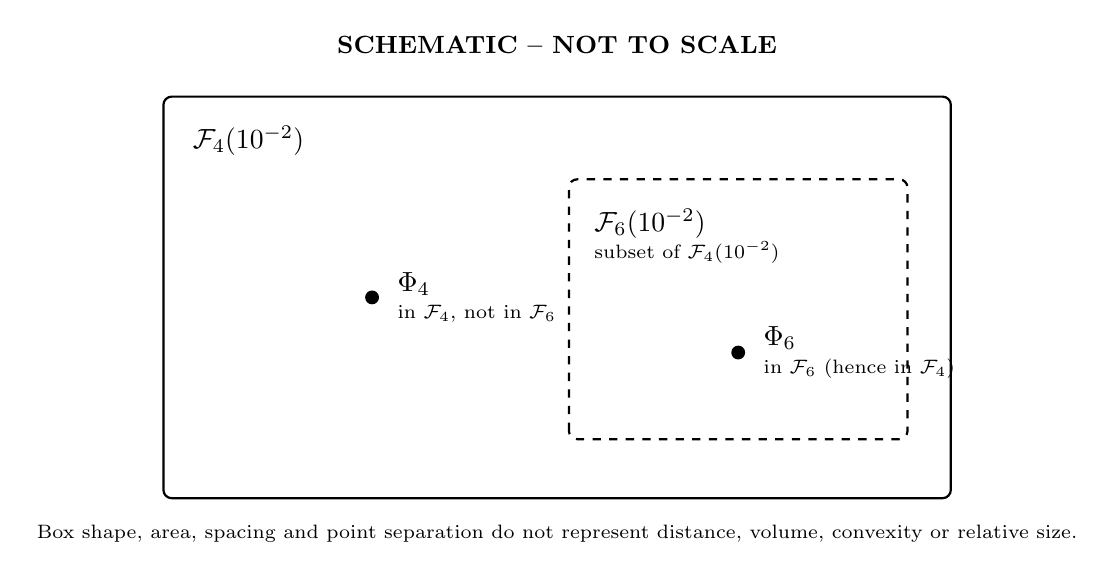
\begin{tikzpicture}[x=1cm,y=1cm]
  \node[font=\small\bfseries] at (0,3.35) {SCHEMATIC -- NOT TO SCALE};
  \draw[thick,rounded corners=3pt] (-5,-2.4) rectangle (5,2.7);
  \node[anchor=north west] at (-4.75,2.45) {$\mathcal F_4(10^{-2})$};

  \draw[thick,dashed,rounded corners=3pt] (0.15,-1.65) rectangle (4.45,1.65);
  \node[anchor=north west,align=left] at (0.35,1.40)
    {$\mathcal F_6(10^{-2})$\\[-2pt]\scriptsize subset of $\mathcal F_4(10^{-2})$};

  \fill (-2.35,0.15) circle (2.5pt);
  \node[anchor=west,align=left] at (-2.15,0.15)
    {$\Phi_4$\\[-2pt]\scriptsize in $\mathcal F_4$, not in $\mathcal F_6$};

  \fill (2.30,-0.55) circle (2.5pt);
  \node[anchor=west,align=left] at (2.50,-0.55)
    {$\Phi_6$\\[-2pt]\scriptsize in $\mathcal F_6$ (hence in $\mathcal F_4$)};

  \node[align=center,font=\scriptsize] at (0,-2.85)
    {Box shape, area, spacing and point separation do not represent distance, volume, convexity or relative size.};
\end{tikzpicture}
